\documentclass{article}
\usepackage[utf8]{inputenc}
\usepackage{amsmath, amssymb, amsthm}
\usepackage[margin=1in]{geometry}
\usepackage{graphicx}  % For including images
\usepackage{listings}  % For including code
\usepackage{xcolor}  % For code highlighting
\usepackage{subcaption}  % For subfigures
\usepackage{hyperref}
\usepackage{tikz}
\usepackage{pdfpages}
\usepackage{tikz}
\usepackage{graphicx}
\usepackage{algorithm}
\usepackage{algpseudocode}

\usetikzlibrary{shapes.geometric, arrows}

\tikzstyle{startstop} = [rectangle, rounded corners, minimum width=2.5cm, minimum height=1cm, text centered, draw=black, fill=red!30]
\tikzstyle{process} = [rectangle, minimum width=3cm, minimum height=1cm, text centered, draw=black, fill=blue!20]
\tikzstyle{decision} = [diamond, minimum width=2cm, minimum height=1cm, text centered, draw=black, fill=green!30]
\tikzstyle{arrow} = [thick,->,>=stealth]


\usetikzlibrary{positioning}

% Define theorem environments
\newtheorem{theorem}{Theorem}
\newtheorem{lemma}{Lemma}
\newtheorem{definition}{Definition}
\newtheorem{corollary}{Corollary}
% Define custom solution environment
\newenvironment{solution}{\noindent\textbf{Solution:} }{\qed}
% Code listing style
\lstset{
    language=Python,
    basicstyle=\ttfamily\footnotesize,
    keywordstyle=\color{blue},
    commentstyle=\color{gray},
    stringstyle=\color{red},
    breaklines=true,
    numbers=left,
    numberstyle=\tiny\color{gray},
    frame=single
}
\usetikzlibrary{positioning, shapes, arrows.meta}

\title{ECE-GY 7123 Advanced Machine Learning \\ \Large Homework 3}
\author{Ali Hamza (ah7072)}
\date{\today}

\begin{document}
\maketitle

\section*{Problem 1}
\subsection*{Kernel Logistic Regression}
We will implement Kernel Logistic Regression with \(L_2\) regularization. The objective function is:
\begin{equation}
    J(\omega) = -\sum_{i=1}^{N} \log\Bigl(\sigma\bigl(y_i\,\omega^T k_i\bigr)\Bigr) + \lambda\, \omega^T\omega,
\end{equation}
where \(y_i\) is the label of data point \(x_i\), and \(k_i\) is defined as
\begin{equation}
    k_i = \begin{bmatrix} k(x_i, x_1) \\ k(x_i, x_2) \\ \vdots \\ k(x_i, x_N) \end{bmatrix}.
\end{equation}
The sigmoid function is given by
\begin{equation}
    \sigma(z) = \frac{1}{1 + e^{-z}}.
\end{equation}
We use the RBF kernel:
\begin{equation}
    k(x, x') = \exp\!\left(-\frac{\|x - x'\|^2}{2\sigma^2}\right),
\end{equation}
with the bandwidth parameter set by the heuristic
\begin{equation}
    \sigma^2 = \frac{1}{N^2} \sum_{i,j=1}^{N}\|x_i - x_j\|^2.
\end{equation}
  After computing \(\omega\), for a new data point \(x\) we form
\begin{equation}
    k(x) = \begin{bmatrix} k(x, x_1) \\ k(x, x_2) \\ \vdots \\ k(x, x_N) \end{bmatrix},
\end{equation}
and predict
\begin{equation}
    p(y=1\mid x) = \sigma\bigl(\omega^T k(x)\bigr).
\end{equation}
The class prediction is
\begin{equation}
  \hat{y} = \begin{cases}
    1, & \text{if } p(y=1\mid x) \geq 0.5, \\
    -1, & \text{if } p(y=1\mid x) < 0.5.
  \end{cases}
\end{equation}
Given that there is no closed form solution for \(\omega\), we will use an optimizer to minimize the objective function. We will use a variety of optimizers: (1) Gradient Descent, (2) Stochastic Gradient Descent, (3) BFGS, and (4) L-BFGS. The code for the optimizers is provided in the next section.

\subsection*{Optimizers}

We start with the objective function
\[
J(\omega) = -\sum_{i=1}^{N} \log\Bigl(\sigma\bigl(y_i\,\omega^T k_i\bigr)\Bigr) + \lambda\,\omega^T\omega,
\]
with the sigmoid defined as
\[
\sigma(z)=\frac{1}{1+e^{-z}}, \quad \text{and} \quad z_i = y_i\,\omega^T k_i.
\]
Differentiating \(-\log(\sigma(z_i))\) with respect to \(z_i\) yields
\[
\frac{d}{dz_i}\Bigl[-\log\bigl(\sigma(z_i)\bigr)\Bigr] = \sigma(z_i)-1.
\]
Since \(\nabla_\omega z_i = y_i\,k_i\), by the chain rule we have for each \(i\)
\[
\nabla_\omega\Bigl[-\log\bigl(\sigma(z_i)\bigr)\Bigr] = \bigl(\sigma(z_i)-1\bigr)y_i\,k_i.
\]
Summing over all data points and including the regularization term, the full gradient is
\[
\nabla J(\omega) = \sum_{i=1}^{N} \bigl(\sigma(y_i\,\omega^T k_i)-1\bigr)y_i\,k_i + 2\lambda\,\omega,
\]
or equivalently,
\[
\nabla J(\omega) = -\sum_{i=1}^{N} \Bigl(1-\sigma(y_i\,\omega^T k_i)\Bigr)y_i\,k_i + 2\lambda\,\omega.
\]

\subsubsection*{a. Gradient Descent}

The update rule is given by
\[
\omega^{(t+1)} = \omega^{(t)} - \eta\, \nabla J(\omega^{(t)}),
\]
where \(\eta > 0\) is the learning rate.

\begin{algorithm}
  \caption{Gradient Descent for Kernel Logistic Regression}
  \begin{algorithmic}[1]
  \Require Training data $\{(x_i, y_i)\}_{i=1}^{N}$, learning rate $\eta$, regularization parameter $\lambda$, tolerance $\epsilon$, maximum iterations $T$
  \State Initialize $\omega \gets 0$, $t \gets 0$
  \Repeat
      \State Compute gradient:
      \[
        g \gets -\sum_{i=1}^{N}\Bigl(1-\sigma\bigl(y_i\,(\omega^\top k_i)\bigr)\Bigr)y_i\,k_i + 2\lambda\,\omega
      \]
      \State Update: $\omega \gets \omega - \eta\, g$
      \State Increment: $t \gets t+1$
  \Until{$\|g\| < \epsilon$ \textbf{or} $t \ge T$}
  \State \Return $\omega$
  \end{algorithmic}
\end{algorithm}

\subsubsection*{b. Stochastic Gradient Descent}

Instead of computing the gradient over the full dataset, SGD approximates it using a single (or a mini-batch of) data sample(s) per iteration.

\begin{algorithm}[H]
  \caption{Stochastic Gradient Descent for Kernel Logistic Regression}
  \begin{algorithmic}[1]
  \Require Training data $\{(x_i,y_i)\}_{i=1}^N$, learning rate $\eta$, regularization parameter $\lambda$, tolerance $\epsilon$, maximum iterations $T$
  \State Initialize $\omega \gets 0$, $t \gets 0$
  \Repeat
      \State Shuffle the training data $\{(x_i,y_i)\}_{i=1}^N$
      \For{each sample $(x_i,y_i)$ in the shuffled data}
          \State Compute the kernel vector: 
          \[
            k_i \gets [k(x_i,x_1),\, k(x_i,x_2),\, \dots,\, k(x_i,x_N)]^\top
          \]
          \State Compute the sample gradient:
          \[
            g_i \gets -\Bigl(1-\sigma\bigl(y_i\,(\omega^\top k_i)\bigr)\Bigr)y_i\,k_i
          \]
          \State Update $\omega$:
          \[
            \omega \gets \omega - \eta\left(g_i + \frac{2\lambda}{N}\,\omega\right)
          \]
      \EndFor
      \State Increment $t \gets t+1$
  \Until{convergence criteria met or $t \ge T$}
  \State \Return $\omega$
  \end{algorithmic}
\end{algorithm}

\subsubsection*{c. BFGS}

BFGS is a quasi-Newton method that iteratively updates an estimate of the inverse Hessian matrix to obtain a search direction. It uses both gradient and function evaluations.

\begin{algorithm}[H]
  \caption{BFGS for Kernel Logistic Regression}
  \begin{algorithmic}[1]
  \Require Training data $\{(x_i,y_i)\}_{i=1}^N$, initial parameter vector $\omega$, regularization parameter $\lambda$, tolerance $\epsilon$, maximum iterations $T$
  \State Initialize inverse Hessian estimate: $H \gets I$, set iteration counter $t \gets 0$
  \Repeat
      \State Compute full gradient:
      \[
        g \gets -\sum_{i=1}^{N} \Bigl(1-\sigma\bigl(y_i\,(\omega^\top k_i)\bigr)\Bigr)y_i\,k_i + 2\lambda\,\omega
      \]
      \State Determine search direction:
      \[
        p \gets -H\,g
      \]
      \State Perform line search to determine step size $\alpha$
      \State Update parameters: 
      \[
        \omega_{\text{new}} \gets \omega + \alpha\, p
      \]
      \State Compute new gradient:
      \[
        g_{\text{new}} \gets -\sum_{i=1}^{N} \Bigl(1-\sigma\bigl(y_i\,(\omega_{\text{new}}^\top k_i)\bigr)\Bigr)y_i\,k_i + 2\lambda\,\omega_{\text{new}}
      \]
      \State Set:
      \[
        s \gets \omega_{\text{new}} - \omega,\quad y_{\text{diff}} \gets g_{\text{new}} - g
      \]
      \State Update the inverse Hessian estimate:
      \[
        H \gets \left(I - \frac{s\,y_{\text{diff}}^\top}{y_{\text{diff}}^\top s}\right) H \left(I - \frac{y_{\text{diff}}\,s^\top}{y_{\text{diff}}^\top s}\right) + \frac{s\,s^\top}{y_{\text{diff}}^\top s}
      \]
      \State Set $\omega \gets \omega_{\text{new}}$, $g \gets g_{\text{new}}$
      \State Increment $t \gets t+1$
  \Until{$\|g\| < \epsilon$ \textbf{or} $t \ge T$}
  \State \Return $\omega$
  \end{algorithmic}
\end{algorithm}

\subsubsection*{d. L-BFGS}

L-BFGS is a limited-memory variant of BFGS that stores only a few vectors from previous iterations to approximate the inverse Hessian, making it suitable for high-dimensional problems.

\begin{algorithm}[H]
  \caption{L-BFGS for Kernel Logistic Regression}
  \begin{algorithmic}[1]
  \Require Training data $\{(x_i, y_i)\}_{i=1}^{N}$, initial parameter vector $\omega$, regularization parameter $\lambda$, tolerance $\epsilon$, maximum iterations $T$, memory size $m$
  \State Initialize $\omega$, set iteration counter $t \gets 0$
  \State Initialize empty lists: $S \gets []$ and $Y \gets []$ \Comment{$S$ stores past update vectors $s$, and $Y$ stores gradient differences $y$}
  \Repeat
      \State Compute full gradient:
      \[
        g \gets -\sum_{i=1}^{N}\Bigl(1-\sigma\bigl(y_i\,(\omega^\top k_i)\bigr)\Bigr)y_i\,k_i + 2\lambda\,\omega
      \]
      \State \textbf{// Two-loop recursion to compute search direction}
      \State Set $q \gets g$
      \For{$i = |S| \text{ downto } 1$} \Comment{Iterate from the most recent to the oldest}
          \State $\rho_i \gets 1 / \bigl(Y_i^\top S_i\bigr)$
          \State $\alpha_i \gets \rho_i \cdot \bigl(S_i^\top q\bigr)$
          \State $q \gets q - \alpha_i\,Y_i$
      \EndFor
      \State Set initial Hessian approximation $H_0 \gets \gamma I$ \Comment{Often, $\gamma$ is chosen as $\frac{S_{|S|}^\top Y_{|S|}}{Y_{|S|}^\top Y_{|S|}}$}
      \State Compute $r \gets H_0\, q$
      \For{$i = 1 \text{ to } |S|$} \Comment{Iterate from the oldest to the most recent}
          \State $\beta_i \gets \rho_i \cdot \bigl(Y_i^\top r\bigr)$
          \State $r \gets r + S_i\,(\alpha_i - \beta_i)$
      \EndFor
      \State Set search direction $p \gets -r$
      \State Perform line search to find step size $\alpha$
      \State Update: $\omega_{\text{new}} \gets \omega + \alpha\, p$
      \State Compute new gradient:
      \[
        g_{\text{new}} \gets -\sum_{i=1}^{N}\Bigl(1-\sigma\bigl(y_i\,(\omega_{\text{new}}^\top k_i)\bigr)\Bigr)y_i\,k_i + 2\lambda\,\omega_{\text{new}}
      \]
      \State Set $s_{\text{new}} \gets \omega_{\text{new}} - \omega$
      \State Set $y_{\text{new}} \gets g_{\text{new}} - g$
      \If{length($S$) = $m$}
          \State Discard the oldest vectors from $S$ and $Y$
      \EndIf
      \State Append $s_{\text{new}}$ to $S$ and $y_{\text{new}}$ to $Y$
      \State Set $\omega \gets \omega_{\text{new}}$, $g \gets g_{\text{new}}$
      \State Increment $t \gets t + 1$
  \Until{$\|g\| < \epsilon$ \textbf{or} $t \ge T$}
  \State \Return $\omega$
  \end{algorithmic}
\end{algorithm}

\subsection*{Implementation}
The code for the optimizers is provided in the following sections. The implementation includes functions for each optimizer, as well as a function to compute the kernel matrix and the objective function.

\subsection*{Dataset}
The given dataset has two classes, each with 11000 samples with labels 1 and -1. The dataset is split into training and testing sets, with 1000 samples in the test set. The training set is used to train the model, and the test set is used to evaluate its performance. The dataset has the following characteristics:

\begin{figure}
\centering  
\begin{verbatim}
          --- Data Summary ---
          Name               Size                Bytes  Class     Attributes

          TestX           1000x784             6272000  double              
          TestY           1000x1                  8000  double              
          TrainingX      10000x784            62720000  double              
          TrainingY      10000x1                 80000  double              

          --- Training Data ---
          TrainingX: 10000 x 784
          TrainingY: 10000 x 1

          --- Test Data ---
          TestX: 1000 x 784
          TestY: 1000 x 1

          ---Unique labels in Training/TestY---
              -1
              1

          Warning: Columns of X are linearly dependent to within machine precision.
          Using only the first 674 components to compute TSQUARED. 
          Variance explained by PC1: 10.56%
          Variance explained by PC2: 7.70%
\end{verbatim}
  \caption{Dataset summary}
  \label{fig:dataset_summary}
\end{figure}


\begin{figure}[H]
  \centering
  \begin{subfigure}[b]{0.45\textwidth}
    \centering
    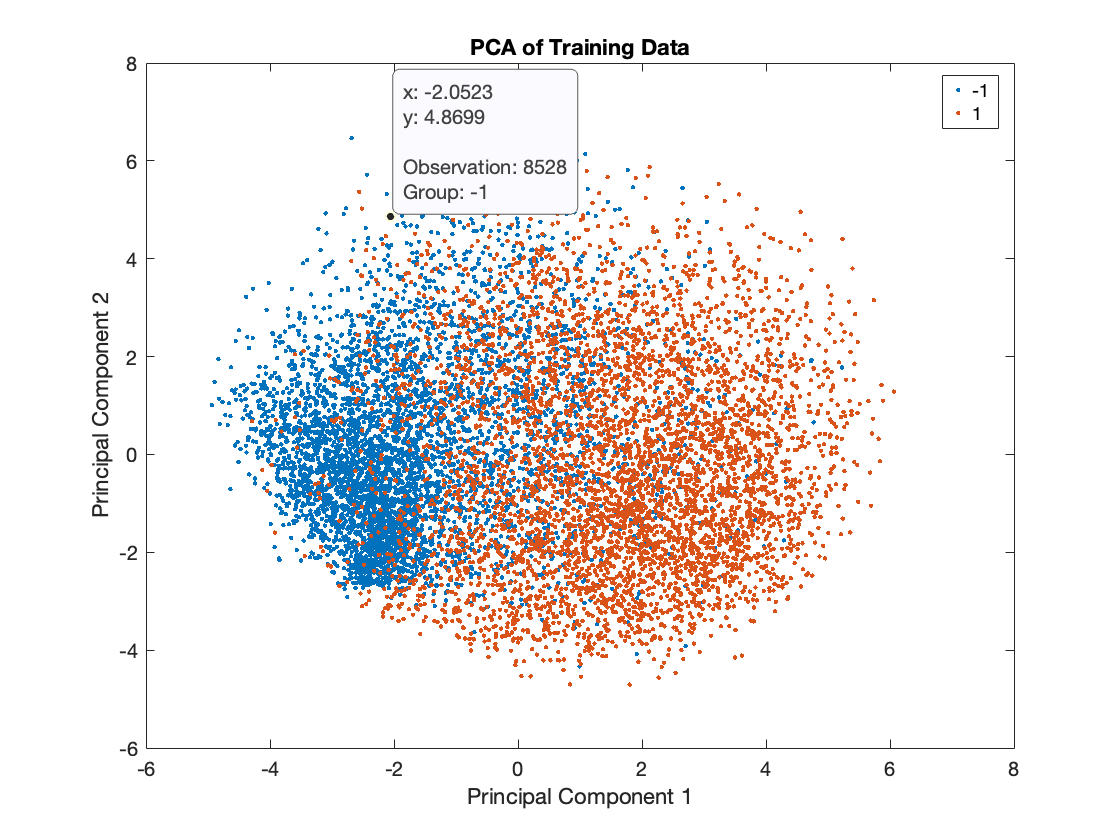
\includegraphics[width=\textwidth]{images/train_data.png}
    \caption{Training data distribution.}
    \label{fig:train_data}
  \end{subfigure}
  \begin{subfigure}[b]{0.45\textwidth}
    \centering
    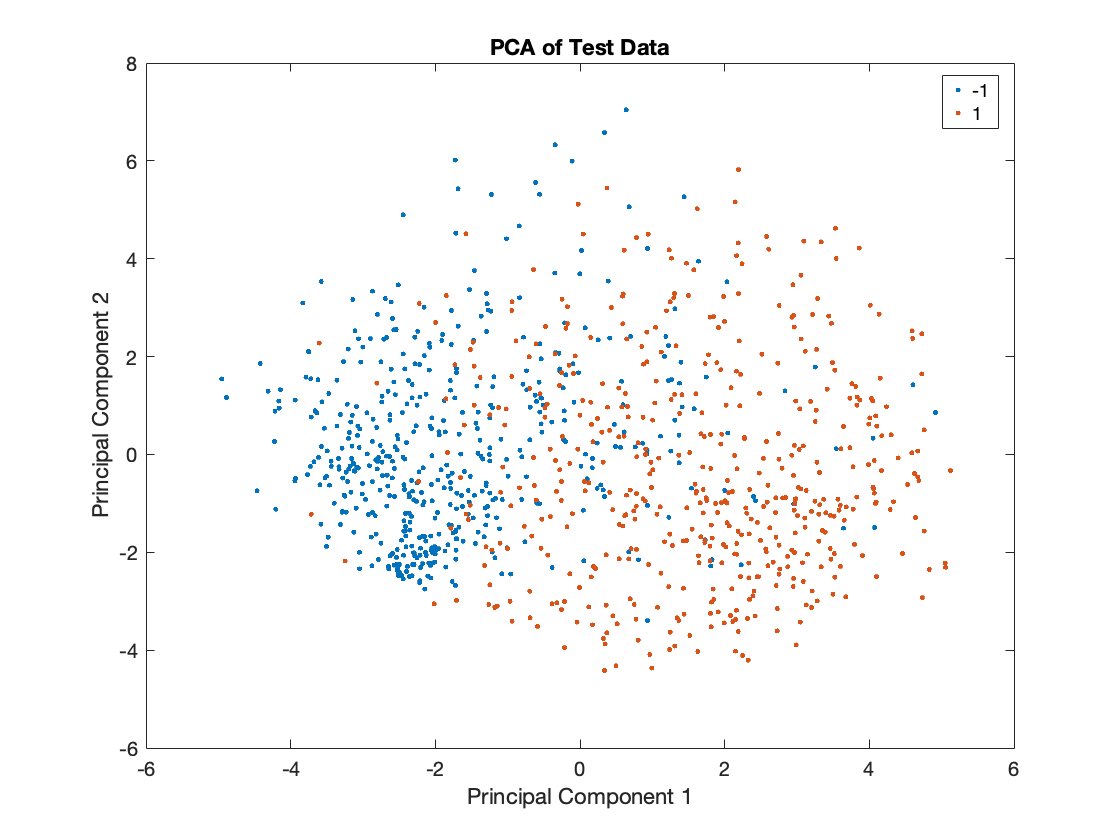
\includegraphics[width=\textwidth]{images/test_data.png}
    \caption{Test data distribution.}
    \label{fig:test_data}
  \end{subfigure}
  \caption{PCA projection of the training and test data}
  \label{fig:side_by_side_images}
\end{figure}


\subsection*{Results}


\newpage
\section*{Appendix}
\subsection*{Dataset Code}

\lstinputlisting[language=Matlab]{/Users/aliha/Library/CloudStorage/OneDrive-Personal/nyu/tandon/spring-2025/ece-gy-7123-advml/hw3/code/data.m}


\end{document}
